%%%%%%%%%%%%%%%%%%%%%%%%%%%%%%%%%%%%%%%%%%%%%%%%%%%%%%%%%%%%%%%%%%%%%%%%%%%%%%%%
%%%%%%%%%%%%%%%%%%   Vorlage für eine Abschlussarbeit   %%%%%%%%%%%%%%%%%%%%%%%%
%%%%%%%%%%%%%%%%%%%%%%%%%%%%%%%%%%%%%%%%%%%%%%%%%%%%%%%%%%%%%%%%%%%%%%%%%%%%%%%%

% Erstellt von Maximilian Nöthe, <maximilian.noethe@tu-dortmund.de>
% ausgelegt für lualatex und Biblatex mit biber

% Kompilieren mit 
% lualatex dateiname.tex
% biber dateiname.bcf
% lualatex dateiname.tex
% lualatex dateiname.tex
% oder einfach mit:
% make

\documentclass[
  BCOR=12mm,     % 12mm binding corrections, adjust to fit your binding
  parskip=half,  % new paragraphs start with half line vertical space
  open=any,      % chapters start on both odd and even pages
  cleardoublepage=plain,  % no header/footer on blank pages
]{tudothesis}


% Warning, if another latex run is needed
\usepackage[aux]{rerunfilecheck}

% just list chapters and sections in the toc, not subsections or smaller
\setcounter{tocdepth}{1}

%------------------------------------------------------------------------------
%------------------------------ Sprache und Schrift: --------------------------
%------------------------------------------------------------------------------
\usepackage{fontspec}
\defaultfontfeatures{Ligatures=TeX}  % -- becomes en-dash etc.

% german language
\usepackage{polyglossia}
\setdefaultlanguage{english}

% for english abstract and english titles in the toc
\setotherlanguages{english}

% intelligent quotation marks, language and nesting sensitive
\usepackage[autostyle]{csquotes}

% microtypographical features, makes the text look nicer on the small scale
\usepackage{microtype}

%------------------------------------------------------------------------------
%------------------------ Für die Matheumgebung--------------------------------
%------------------------------------------------------------------------------

\usepackage{amsmath}
\usepackage{amssymb}
\usepackage{mathtools}

% Enable Unicode-Math and follow the ISO-Standards for typesetting math
\usepackage[
  math-style=ISO,
  bold-style=ISO,
  sans-style=italic,
  nabla=upright,
  partial=upright,
]{unicode-math}
\setmathfont{Latin Modern Math}

% nice, small fracs for the text with \sfrac{}{}
\usepackage{xfrac}  


%------------------------------------------------------------------------------
%---------------------------- Numbers and Units -------------------------------
%------------------------------------------------------------------------------

\usepackage[
  locale=UK,
  separate-uncertainty=true,
  per-mode=symbol-or-fraction,
]{siunitx}
\sisetup{math-micro=\text{µ},text-micro=µ}

%------------------------------------------------------------------------------
%-------------------------------- tables  -------------------------------------
%------------------------------------------------------------------------------

\usepackage{booktabs}       % stellt \toprule, \midrule, \bottomrule

%------------------------------------------------------------------------------
%-------------------------------- graphics -------------------------------------
%------------------------------------------------------------------------------

\usepackage{graphicx}
\usepackage{grffile}

% allow figures to be placed in the running text by default:
\usepackage{scrhack}
\usepackage{float}
\floatplacement{figure}{htbp}
\floatplacement{table}{htbp}

% keep figures and tables in the section
\usepackage[section, below]{placeins}


%------------------------------------------------------------------------------
%---------------------- customize list environments ---------------------------
%------------------------------------------------------------------------------

\usepackage{enumitem}

%------------------------------------------------------------------------------
%------------------------------ Bibliographie ---------------------------------
%------------------------------------------------------------------------------

\usepackage[
  backend=biber,   % use modern biber backend
  sorting=none,
  style=numeric-comp,
  autolang=hyphen, % load hyphenation rules for if language of bibentry is not
                   % german, has to be loaded with \setotherlanguages
                   % in the references.bib use langid={en} for english sources
]{biblatex}
\addbibresource{references.bib}  % die Bibliographie einbinden
\DefineBibliographyStrings{german}{andothers = {{et\,al\adddot}}} 

%------------------------------------------------------------------------------
%------------------------------ Sonstiges: ------------------------------------,linkbordercolor=tugreen
%------------------------------------------------------------------------------

%\usepackage[pdfusetitle,unicode]{hyperref}
\usepackage{bookmark}
\usepackage[shortcuts]{extdash}
\usepackage{atlasphysics}
\usepackage{units}
\usepackage{amssymb}
\usepackage{tikz-feynman}
\usepackage{tabularx} 


 
%multi-row
\usepackage{multirow}

\renewbibmacro{in:}{}

\catcode`\_=\active
\def_#1{\sb{\text{#1}}}

%------------------------------------------------------------------------------
%-------------------------    Angaben zur Arbeit   ----------------------------
%------------------------------------------------------------------------------

\author{Stella Oppermann}
\title{Optimization Studies for the Boosted Event Selection in a Search for Vector-Like Quark Pair Production in the Channels TT\texorpdfstring{$\longrightarrow$}~WbZt and BB\texorpdfstring{$\longrightarrow$}~WtZb with the ATLAS Experiment}
\date{Juli 2016} 
\birthplace{Greven}
\chair{Lehrstuhl für Experimentelle Physik IV}
\division{Fakultät Physik}
\thesisclass{Bachelor of Science}
\submissiondate{18. Juli 2016}
\firstcorrector{Prof. Dr. Kevin Kröninger}
\secondcorrector{Priv.-Doz. Dr. Reiner Klingenberg}

% tu logo on top of the titlepage
\titlehead{\includegraphics[height=1.5cm]{logos/tu-logo.pdf}}

\begin{document}
\frontmatter
%\thispagestyle{empty}
\setcounter{page}{2}
\section*{Hinweise}
Empfohlen wird die Verwendung dieser Vorlage mit der jeweils aktuellsten TeXLive Version (Linux, Windows) bzw. MacTeX Version (MacOS).
Aktuell ist dies TeXLive 2015. Download hier:
\begin{center}
  \ttfamily\url{https://www.tug.org/texlive/}
\end{center}
Bei Verwendung von TexLive Versionen 2014 und älter sollte
die Zeile
\begin{center}
\verb+\RequirePackage{fixltx2e}+ 
\end{center}
als erste Zeile der Präambel noch vor der Dokumentenklasse eingefügt werden.
Dies lädt diverse Bugfixes für LaTeX, die ab TexLive 2015 Standard sind.

Die Vorlage \texttt{thesis.tex} ist für die Kompilierung mit \texttt{lualatex} ausgelegt, mit wenigen Anpassungen kann sie aber auch mit \texttt{pdflatex} oder \texttt{xelatex} verwendet werden. 
Die Dokumentenklasse \texttt{tudothesis.cls} kann mit allen drei Programmen verwednet werden.

Achten Sie auch auf die Kodierung der Quelldateien.
Bei Verwendung von Xe\LaTeX\ oder Lua\LaTeX\ (empfohlen) müssen die
Quelldateien UTF-8 kodiert sein.
Bei Verwendung von pdf\LaTeX\ nutzen Sie die Pakete \texttt{inputenc} und \texttt{fontenc} mit der korrekten Wahl der Kodierungen.

Eine aktuelle Version dieser Vorlage steht unter 
\begin{center}
  \ttfamily\url{https://github.com/maxnoe/tudothesis}
\end{center}
zur Verfügung.

Alle verwendeten Pakete werden im \LaTeX{} Kurs von Pep et al.\ erklärt:
\begin{center}
  \ttfamily\url{http://toolbox.pep-dortmund.org/notes}
\end{center}

Für Rückmeldungen und bei Problemen mit der Klasse oder Vorlage, bitte ein \emph{Issue} auf GitHub aufmachen oder eine Email an
\href{mailto:maximilian.noethe@tu-dortmund.de}{maximilian.noethe@tu-dortmund.de} schreiben.

Wenn Sie die Dokumentenklasse mit der Option \texttt{tucolor} laden, werden verschiedene Elemente in TU-Grün gesetzt.

\maketitle

% Gutachterseite
\makecorrectorpage

% hier beginnt der Vorspann, nummeriert in römischen Zahlen
\thispagestyle{plain}

\section*{Kurzfassung}
Hier steht eine Kurzfassung der Arbeit in deutscher Sprache inklusive der Zusammenfassung der
Ergebnisse.
Zusammen mit der englischen Zusammenfassung muss sie auf diese Seite passen.

\section*{Abstract}
\begin{english}
The abstract is a short summary of the thesis in English, together with the German summary it has to fit on this page.
\end{english}

\tableofcontents

\mainmatter
% Hier beginnt der Inhalt mit Seite 1 in arabischen Ziffern
\chapter{Motivation for a Search for Vector-Like Quarks}




\section{Short Overview of the Standard Model of Particle Physics}
Particle physics deals with elementary particles without any substructure and bound states of the elemantary particles forming other particles.
Moreover the interactions between the particles  are considered.
Table \ref{standardmodel} shows the different elementary particles the Standard Model consists of.

\begin{table}
\centering
%\setlength{\tabcolsep}{3cm}
\begin{tabular}{|c|c c c|c|} 
\hline
 & 1st Generation & 2nd Generation & 3rd Generation &  Bosons \\
\hline
\hline
&	&	&	& \small{Vector-bosons}	\\
Quarks &  $\begin{matrix} u \\ \\ d \end{matrix}$ & $\begin{matrix} c \\ \\ s \end{matrix}$ & $\begin{matrix} t \\ \\ b \end{matrix}$ & $\gamma$ \\
& & & & g  \\
&	&	&	&	\\
& &  &  & $W^{\pm}$, $Z^{0}$ \\
Leptons & $\begin{matrix} \nu_{e} \\ \\ e \end{matrix}$ & $\begin{matrix} \nu_{\mu} \\ \\ \mu \end{matrix}$ & $\begin{matrix} \nu_{\tau} \\ \\ \tau \end{matrix}$ & \small{Scalar boson}  \\
&	&	&	&   H \\
&	&	&	&     \\
 \hline
\end{tabular}
\caption{Elemantary particles of the Standard Model.}
\label{standardmodel}
\end{table}



Both leptons and quarks are fermions with spin $s= \frac{1}{2}$. 
There are twelve fermions, with one anti-particle for each fermion, which are segmented in three generations.     
For the leptons there is a lepton with charge $q = -1$ (electron e, muon $\mu$, tau $\tau$) and a corresponding neutrino without electric charge(electron-neutrino $\nu_{e}$, muon-neutrino $\nu_{\mu}$, tau-neutrino $\nu_{\tau}$) in each genaration.
The mass of charged leptons increases with the generation in which it is located and the neutrinos are supposed to be massless.\\
Quark are elementary particles which can not be observed in unbound states.
The quarks can be divided in up-type and down-types with charge $q = +\frac{2}{3}$ for the up- and $q = -\frac{1}{3}$ for the down-types.
Upquark u, charmequark c and topquark t are up-types while downquark d, strangequark s and bottomquark b are down-type quarks. 
The mass of the quarks increases with the generation like it was mentioned for the leptons and the down-types are heavier than the up-types exept for the first generation.
The topquark is of peculiar interest because it is the heaviest patricles of the Standard Model and unlike every other quark don't occur in bound states.
Furthermore the standard model includes particles with spin 1 which are the gauge bosons.
They include the photon $\gamma$,the gluons g, the W bosons $W^{\pm}$ and the Z boson $Z^{0}$.
The gauge bosons are the mediators of the fundamental forces. 
The photon $\gamma$ mediates the elektromagnetic, the gluons the strong  and the $W^{\pm}$ and $Z^{0}$ the weak force.  
Fermions and particles, which are bound states of the fermions, interact via the fundamental forces.
There are different characteristics particles have to fulfill to participate in the different interactions.
Particles with electric charge can interact via the electromagnetic force.
The strong interaction occurs between particles with colour charge, which are quarks, bound states of quarks and gluons itself.
The weak force is mediated between particles with weak charge having a left-handed chirality.\\
The $\gamma$ and the gluons are massless, while the $W^{\pm}$ and $Z^{0}$ carry mass. 
W bosons are the only gauge bosons which have electric charge with +1 for the $W^{+}$ and -1 for the $W^{-}$.\\
Finally there is a scalar boson with spin 0, the higgs boson H.
The higgs carries mass but no electric charge.
It was predicted  by the higgs mechanism.
The mechanism explains the existence of mass for the elementary particles of the Standard Model.




\section{Beyond Standard Model Physics: Vector-like Quarks}
Vector-like quarks \cite{handbook} are predicted as fermions with spin $\frac{1}{2}$.
There are four types of vector-like quarks which are assumed to couple only to the third generation standard model quarks.
Caused by the coupling between the vector-like quarks and the third generation quarks the coupling of the Standard model quarks to the vector bosons would change.\\
The different vector-like quarks appear in seven multiplets of which two are singulets, three doublets and two triplets.
Table \ref{vectorlikequarks} lists the different types of vector-like quarks with their specific charge and the possible multiplets they can be assigned too.

\begin{table}
\centering
\begin{tabular}{|c|c||c|} 
\hline
Flavor& Charge & Arragnement in multiplets\\
\hline
  & 	           & \multirow{3}{*}{$T^{0}_{L,R}$ , $B^{0}_{L,R}$ (singlets)}\\
T & $+\sfrac{2}{3}$ & \multirow{4}{*}{(X $T^{0})_{L,R}$,  ($T^{0} B^{0})_{L,R}$, ($B^{0} Y)_{L,R}$ (doublets)} \\
B & $-\sfrac{1}{3}$ & \\
Y & $+\sfrac{5}{3}$ & \multirow{3}{*}{(X $T^{0} B^{0} )_{L,R}$,  ($T^{0} B^{0} Y)_{L,R}$ (triplets)} \\  
X & $-\sfrac{4}{3}$ & \\
  &                &\\
\hline
\end{tabular}
\caption{Containing the different types of vector-like quarks with their specific charge and the possible arragnement in multiplets. 
The zero superscript is used to denote the weak eigenstates and seperate them from the mass eigenstates.
For the multiplets containing X and Y the mass and weak eigenstates are the same. }
\label{vectorlikequarks}
\end{table}

In this analysis only the singulets are considered.\\
Possible decay channels for the vector-like quarks include a combination of the vector bosons or the higgs and a third generation quarks in order that conversation of charge is preexisting.\\
Unlike the Standard Model quarks coupling with a (V-A) (vector minus axialvector) structure regarding the weak interaction, the vector-like quark have purely vector couplings.
Therfore also vector-like quarks with right-handed chirality couple to the weak force.
Because of this tranformation behavior explicit mass term in the lagrangian are not forbidden because they do not break the gauge invariance.
Hence the vector-like quarks don't receive their masses from the higgs mechanism contrary to the Standard Model quarks.\\
If the vector-like quarks would be added to the Standard Model they would offer the possibility to allow tree-level flavour-changing neutral currents and to break the GIM mechanism \cite{GIM}.
Moreover vector-like quarks would provide new origins of CP violation \cite{CP1}, \cite{CP2}.
Vector-like quarks are part of  theories beyond the Standard Model. 
They are for example a necessary part of theories predicting the higgs as pseudo-Goldstone boson to explain why the mass of the higgs is as light as observed \cite{Th1-Th3}. 
Furthermore they are part of the partial-compositeness theory of flavour in which they have an apperence as fermion resonances \cite{Th4,Th5}.
This ideas are used for example in little higgs and composite higgs models .\\
Vector-like quarks can be both pair and single produced.
In this analysis the pair production process approached which is performed with gluon fusion.
The feynman diagramms for both the production process and the specific decay topology considered in this analysis are presented in figure \ref{feynmantts} for the vector-like top and \ref{feynmanbbs} for the vector-like bottom quark. .

\begin{figure}[h!]
\centering
\includegraphics[width=11cm]{figures/tts.pdf}
\caption{Feynman diagramm for the vector-like top production process and decay channel.}
\label{feynmantts}
\end{figure}

\newpage

\begin{figure}[h!]
\centering
\includegraphics[width=11cm]{figures/bbs.pdf}
\caption{Feynman diagramm for the vector-like bottom production process and decay channel.}
\label{feynmanbbs}
\end{figure}

The analysis is in the dilepton channel therefore all particles except the Z boson decay hadronically and form jets. 
The considered decay topology contains tree-level flavour-changing neutral currents.\\
Previous analysis in the di- and trilepton channel with $\sqrt{s}$ = \SI{8}{TeV} for both pair and single production processes set mass limits for the vector-like top and bottom quark\cite{8tevanalysis}. 
The limits for the singulets are $m_{T} >$ \SI{655}{GeV} for the vector-like top and $m_{B} >$ \SI{685}{GeV} for the vector-like bottom quark.  
This limits are at the $95 \%$ confidence level \cite{confidencelevel}.
 











% kapitel2.tex
\chapter{The ATLAS Detector at the LHC}

\section{The LHC}
The LHC \cite{LHC} is a large hadron and lead nuclei accelerator and collider at the CERN.
It consists of four preaccelarators and the main accelarator which has a circumference of around \SI{27}{km}. 
In serveral stations of the main accelarator the ATLAS detector and other detectors are placed. 
In the main accelator both beams for the collision are accelerated in opposite direction at the same time.
For accelerated protons both bunches can contain up to $10^{11}$ protons.
Therfore each event includes many proton-proton collusions.
At each detector there is the possibility to bring the different beams together. 
The LHC currenlty reaches a center-of-mass energy of about $\sqrt{s} =$\SI{13}{TeV}. 
High center-of-mass energys are required for producing heavy particles and therefore essential for a search for very massive vector-like quarks.


\section{The ATLAS Detector}
The ATLAS Detector \cite{ATLAS} is a high luminosity experiment of the LHC. 
The construction of the ATLAS Detector is symmetric around the beam axis with cylindrical components and end caps to cover the full solid angle.
For discribing the ATLAS detector a specific coordinate system is generated.
The interaction point is the origin of the coordinate system and the z-axis is parallel to the beam axis while the x-y plane is perpenticular to the beam axis.
The azimuthal angle $\Phi$ is defined as angle around the beam axis while the polar angle $\Theta$ is measured starting from the beam axis. 
Moreover the pseudorapidity is defined according to $\eta = - ln(tan(\nicefrac{\Theta}{2}))$.
With this defined parameters distances in the pseudorapidity-azimuthal angle space can be calculated in the following way $\Delta R = \sqrt{\Delta \eta^{2} + \Delta \Phi^{2}}$.
Figure \ref{ATLAS} shows the cut-away view of the ATLAS Detector.
\begin{figure}[h!]
\centering
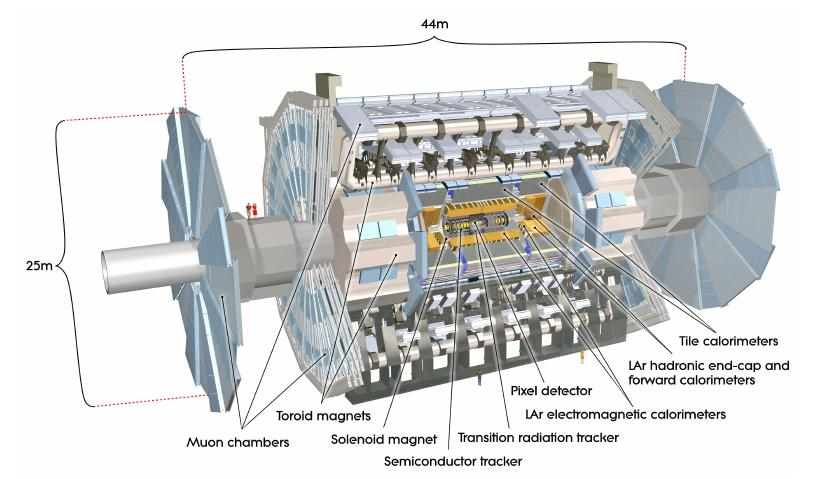
\includegraphics[width=11cm]{figures/atlas.jpg}
\caption{Cut-away view of the ATLAS detector with the different constituents.}
\label{ATLAS}
\end{figure}
There are four main parts the ATLAS detector consists of.
To begin with there is the inner detector which is the first component around the interaction point.
The task of the inner detector is the vertex resolution and furthermore the resolution of the momenta for all charged particles.
It consits of pixel and silicon microstrip detectors trackers and a Transition Radiation Tracker.
A solenoid magnet surrounds the inner detector and immerses it in a magnetic field. 
This causes the curvature of the charged particles tracks and ensures the momentum measurement.\\
The solenoid magnet is surrounded by the electromagnetic and hadronic calorimeters.
The electromagnetic calorimeter is further inside and makes precision measurements of electron and photon energies possible.
Electrons and photons ideally deposit all their energy in the electromagnetic calorimeter by interacting with the detector material.\\
The hadronic calorimeter performs the same goal as the electromagnetic calorimeter for hadrons, which are bound states of the quarks.
Hadrons form jets in the calorimeters.
The particles loose their energy because of hadronic showers in the hadronic calorimeter.
The outermost component of the ATLAS detector is the muon system or muon spectrometer.
For the ideal case only muons reach the muon spectrometer.
The muon spectrometer is immersed with a magnet field resulting from toroid magnets.
The magnets causes the deflection of the muons and enable momentum measurements as mentioned for the inner detector.





% kapitel3.tex
\chapter{Monte-Carlo Samples}

\section{Background Processes}
\label{samples}
In order to perform an unbiased analysis in particle physics, the analysis strategy is studied with simulated samples and only later on compared to data.
In this analysis, only simulated data are considered.
The simulated background samples contain background processes generated with Monte Carlo simulations.
%For the background,  Monte Carlos samples uses random number generators in combination with branching ratios predicted in the Standard Model to simulate processes.
The Monte Carlo samples used in this analysis were passed through a full detector simulation of the ATLAS detector \cite{simulation1, simulation2}.\\
The background is divided into five parts, considering the dominant background processes separately and combining the other backgrounds in one category.
There are the Z+jets backgrounds, which include Z+bottom, Z+charm and Z+light processes.
The Z+bottom process is composed of a Z candidate and a number of b-jets, both are produced at the same time.
The other Z+jets backgrounds are composed similarly, with a number of charm-jets for Z+charm and a number of light-jets (strange-,up-,down-jets).
Moreover, there is the \ttbar{} background, which includes a produced top-quark pair, and the category ``other background'', which contains for example diboson processes, $t \bar{t} e^{+}\!e^{-}$ and $t \bar{t} \mu^{+}\!\mu^{-}$ processes.
The diboson processes include a produced pair of vector bosons (WW, ZW, ZZ) and the $t \bar{t} e^{+}\!e^{-}$ respectively $t \bar{t} \mu^{+}\!\mu^{-}$ processes a associated production of a top-quark pair and a pair of electrons or muons.
Since the different processes and the signal can lead to simular signatures in the detector, caused by partially equal final state products, the processes are considered as main background. \\
The various processes are simulated with different event generators.
Event generators simulate the processes starting from the pp-collision and seperate them into the following stages:
Production of heavy particles , radiation of lighter particles (gluons, photons), decay of heavy unstable particles, hadronization and the decays of the particles resulting from the hadronization into long-lived particles. 
The resulting particles finally enter the detector simulation.
Thereby the production and decay of heavy unstable particles is considered through appropriate matrix elements.
There are event generators, which only generate until the hadronization process and therefore shower programs are added.\\
To simulate the Z+jets samples, the event generator Sherpa 2.2 is used.
Sherpa \cite{Sherpa} performs both the simulation of processes until the hadronization and beyond the hadronization.
Sherpa simulates at leading order precision in $\alpha_{s}$. 
For the \ttbar{} background processes, the generator Powheg is utilized with Pythia 8.1 \cite{Pythia} as shower program.
Powheg \cite{Powheg} is a next-to leading order event generator.
For the diboson background, there are both simulated samples with Sherpa 2.2 and Powheg + Pythia 8.1.
The processes $t \bar{t} e^{+}\!e^{-}$  and $t \bar{t} \mu^{+}\!\mu^{-}$ are simulated with Madgraph as event generator and Pythia 8.1 as shower program.
Madgraph \cite{Madgraph} is a event generator which simulates at leading order.\\
In the analysis the samples are normalized to the value of the integrated luminosity $\int{L} \mathrm{d}t = 3.2 \mathrm{fb}^{-1}$ to provide the possibility of comparing the simulated data with the measured data.\\
In the following analysis, the weighted number of events denote the expected number of events considering the integrated luminosity $\int{L} \mathrm{d}t = 3.2 \mathrm{fb}^{-1}$.


\section{Signal Processes}
The signal also includes processes generated from Monte Carlo simulations. 
In this analysis, both vector-like top and bottom quark are considered to be arranged in the singlet.
The processes are referred to as TTS for the vector-like top quark pair production and BBS for the vector-like bottom quark pair production.
Both TTS and BBS are simulated with the event generator Protos and Pythia 8.1 as shower program.
Protos \cite{Protos} is a leading order event generator.\\
As mentioned in section \ref{samples} for the backround, the samples for the signal are also normalized to the value of the integrated luminosity $\int{L} \mathrm{d}t = 3.2 \mathrm{fb}^{-1}$.
Therefore the weighted number of events also represents the expected number of events for the integrated luminosity $\int{L} \mathrm{d}t = 3.2 \mathrm{fb}^{-1}$.

% kapitel4.tex

\chapter{Preselection in the Boosted Channel}

\section{Event Preselection}
\label{Event Preselection}
For the Monte-Carlo samples used in this analysis a specific preselection is chosen.\\
In table \ref{Event preselection} the different requirements are listed, which are part of this preselection. 

\vspace{0.5cm}

\begin{table}
\centering
\setlength{\tabcolsep}{3cm}
\begin{tabular}{|c|} 
\hline
\textbf{Event preselection} \\
\hline
\hline
\vspace{-0.3cm}
\\
Z boson candidate preselection:\\
\vspace{-0.1cm}
\footnotesize{$\bullet$ pair of opposite sign leptons (same flavor)} \\

\footnotesize{$\bullet$ $\mid m_{l^{+} l^{-}} - m_{Z} \mid$ < \SI{10}{GeV}} \\
\\
\vspace{-0.9cm}
\\
\hline
\vspace{-0.3cm}
\\
$\geq 2$ jets \\
\vspace{-0.4cm}
\\
$\geq$ 2 b-tags\\
\vspace{-0.4cm}
\\
= 2 leptons \\
\hline
\end{tabular}
\caption{Preselection criteria.}
\label{Event preselection}
\end{table}


The first aspect is the Z boson candidate preselection. 
According to the studied leptonic decay channel of the Z boson this includes a reconstructed Z candidate mass with \SI{10}{GeV} around the Z pole resulting from two opposite sign leptons with same flavor.
In this analysis only electrons and muons are considered in the Z candidate reconstruction and not the $\tau$ lepton or neutrinos.
Figure \ref{Zmass} shows the distribution of the reconstructed Z mass. 
Both signal and background are presented in one plot and are normalized to unity. 
The background is illustrated as colour filled histogram with a specific colour for each background process, which is listed in the legend.
The different background processes are stacked, which means that the histograms of the different background processes are added . 
The signal is shown as solid red and blue line for the BBS and TTS process.
In the legend the weighted number of events is displayed in brackets next to each process.
Furthermore the statistical uncertaintys are shown as vertical lines.
The shape of the distribution looks as expected because it displays a pole mass distribution which is smeared because of detector resolution.
Processes including a real Z boson, like the signal and Z+jets processes, have a peak at the Z mass. 
The \ttbar{} background process has no peak at the Z pole mass which is as anticipated as well because the leptons result from independent W boson decays.\\

\begin{figure}
\centering
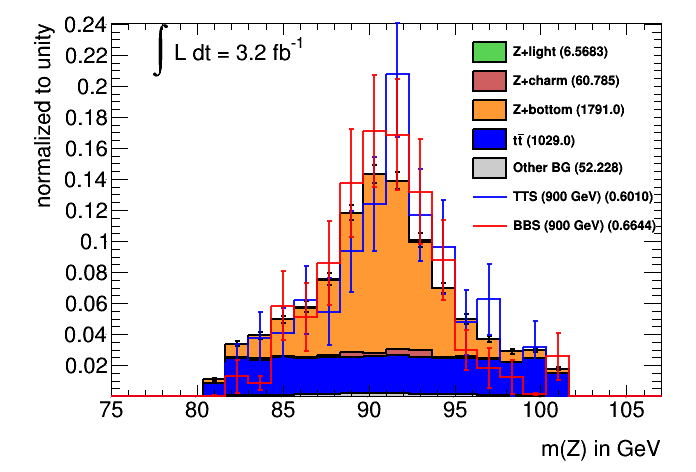
\includegraphics[width=8cm]{figures/Zmass.png}
\caption{Distribution of the reconstructed Z boson mass after the preselection. 
Both signal and background are presented and the distributions are normalized to unity.
The weighted number of events is displayed in the legend in brackets next to the processes. 
The number of events are expected for a integrated luminosity $\int{Ldt}$ = \SI{3,2}{fb^{-1}} }.
\label{Zmass}
\end{figure}

Furthermore, in the preselection at least two jets with $|\eta | < 2.5$ and $p_{T} < \SI{25}{GeV}$ are required.
The $p_{T}$ requirement should ensure that the jets are calibrated and the $\eta$-region is limited because the detector resolution in this $\eta$-region is better than in regions with $|\eta | > 2.5$.  
Because of the specific decay topology, two or more b-tags for the jets are expected.
One b-jet results straight from the vector-like quark decays T\texorpdfstring{$\longrightarrow$}~Wb and B \texorpdfstring{$\longrightarrow$}~Zb.
The other is caused by the third generation top quark decays t\texorpdfstring{$\longrightarrow$}~Wb.
The top quarks are the decay products of the second vector-like quarks with T\texorpdfstring{$\longrightarrow$}~Zt and B\texorpdfstring{$\longrightarrow$}~Wt.\\  
The last aspect of the preselection listed in table \ref{Event preselection}  is the requirement of exact two leptons. 
This guarantee that the analysis is performed in the dilepton channel. There are analysis in the trilepton channel, too.



\section{Boosted Analysis Strategy}
The samples are simulated with a vector-like quark mass of $m_{T/B} =$ \SI{900}{GeV}. 
Because of the massive vector-like T and B the decay products have high transverse momenta. 
Caused by the high transverse momenta the particles of the subsequent decays are strongly collimated. 
This situation is illustrated in figure \ref{boosted} for a top quark decay.
The figure shows the decay for a low and a high top-quark $p_{T}$.
As mentioned before, the figure shows that the decay products of the top-quark are collimated for a high top-quark $p_{T}$.\\

\begin{figure}
\centering
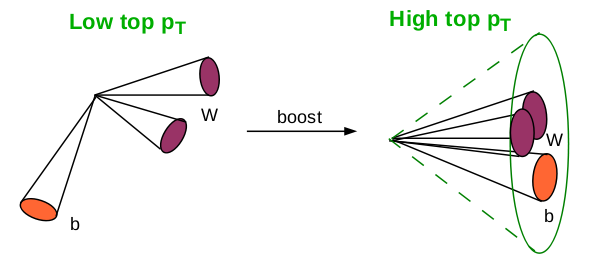
\includegraphics[width=9cm]{figures/boost.png}
\caption{Representative figure for a top quark decay with a high and a low top $p_{T}$ \cite{boosted}.}
\label{boosted}
\end{figure}

This collimated structure of the particles have an inpact on the jet clustering algorithms used in the ATLAS experiment.
Jets can for example be clustered with the anti-$k_{t}$ jet clustering algorithm \cite{antikt}.  
The anti-$k_{t}$ algorithm clusters soft particles around a hard particle within a given radius and forms conical jets. 
If two hard particles are located within an area closer than R, the clustering algorithm is not able to form a smooth circular shape around the hard particles.  
For a low top-quark $p_{T}$, a $R = 0.4$ can be used.
In the high $p_{T}$ regions, it is probable, that the jets from the top decay, which are clustered with $R = 0.4$,  merge because the one decay product can be close to another decay product. 
Hence as mentioned before the anti-$k_{t}$ algorithm is not able to form smooth circular shapes. 
To avoid this problem the boosted analysis strategy can be used for high top-quark transverse momenta.
The idea of the boosted analysis strategy is to cluster one jet which has all decay products of a boosted particle in it.
The area, where the decay products of a particle are located can be estimated with the formula $R \approx \frac{2m}{p_{T}}$, with m and $p_{T}$ for the mass and transverse momentum of the motherparticle and R the distance of the childparticle.
In the boosted analysis a radius of $R = 1.0$ for the cluster algorithm is used. 
A combined result from the top quark mass measurement is $m_{t} =$ \SI{173.34 \pm 0.76}{GeV} \cite{topmass}.
Using the formula mentioned before the boosted analysis is sensibel for a $p_{T}$ of the top quark about \SI{350}{GeV} and more. 
The boosted analysis strategy can be used for a decay of a boosted W boson, too.\\
In this analysis jets clustered with  $R = 1.0$ are used.   
These jets are called large-R jets. 
Large-R jets offer the possibility to introduce top- and boson tagging.
The top-tagger \cite{toptag} utilized in this analysis uses two variables for the top-jet identification, the invariant mass of the jet constituents $m_{jet}$ and the subjettiness ratio $\tau_{32}$, which discribes how adequate the jet can be interpretated as jet with three constuents.
For the analysis the 80\% signal efficiency working point for the top-tagger is choosen. 
The W-tagger \cite {Wtag} works with three substructure variables in combination with a groomed jet mass window.
The chosen working point of the W-tagger has 50\% signal efficiency. 
Table \ref{calibration} contains different conditions large-R jets have to fulfill to ensure that they are calibrated.

\begin{table}[h!]
\centering
\setlength{\tabcolsep}{3cm}
\begin{tabular}{|c|} 
\hline
\textbf{Large-R jet only calibrated for:}\\
\hline
\hline
$p_{T}$(large-R jet) $\geq \SI{200}{GeV}$\\
$\mid \eta \mid < 2.0$ \\
m(large-R jet) $> \SI{50}{GeV}$\\
\hline
\end{tabular}
\caption{Minimum criteria for large-R jets.}
\label{calibration}
\end{table}

Only calibrated large-R jets are considered.
Furthermore large-R jets within an area of $\Delta R < 1.0$ around the Z candidate reconstructed from two electrons are discarded in this analysis.
Figure \ref{deltaR} shows the distribution of the $\Delta R$ between all large-R jets in an event and the Z candidate of this event.

\begin{figure}
\centering
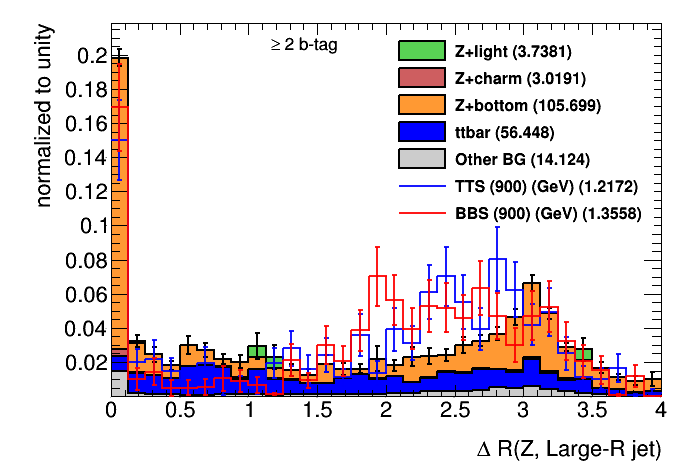
\includegraphics[width=8cm]{figures/deltaR.png}
\caption{Distribution of the $\Delta R$ of the large-R jets and the Z boson candidate after the preselection. 
Both signal and background are presented and the distributions are normalized to unity. 
The weighted number of events is displayed in the legend in brackets next to the processes. 
The number of events are expected for a integrated luminosity $\int L dt$ = \SI{3.2}{fb^{-1}}}.
\label{deltaR}
\end{figure}

The distribution has a clear peak at $\Delta R = 0$, which illustrates that the decay products of the Z candidate are often misidentified as large-R jets.
This is caused by the electrons which can be misidentified as large-R jets because of a simular signature in the detector.
Because of that, it is reasonable to ignore all large-R jets within an area of $\Delta R < 1.0$ around the Z candidate reconstructed from two electrons to avoid that they are treated as large-R jets in the analysis.
This requirement is called overlap removal.



      



\section{Basic Selection Implied by the Boosted WbZt Topology  }
\label{basic selection}
The decay topologys TT \texorpdfstring{$\longrightarrow$}~ZtWb and BB \texorpdfstring{$\longrightarrow$}~ZbWt for the optimization studies in this analysis are defined as mentioned before. 
Because of the specific products of the vector-like quark decays further selection can be added to the preselection discussed in section \ref{Event preselection}.       
It is reasonable that at least two large-R jets should be required considering that there is one top quark and one W boson, which could lead to large-R jets. 
Events without at least one top- and W-tag should also be rejected.  
Figure \ref{ljetmult} shows the multiplicity of the large-R jets.

\begin{figure}
\centering
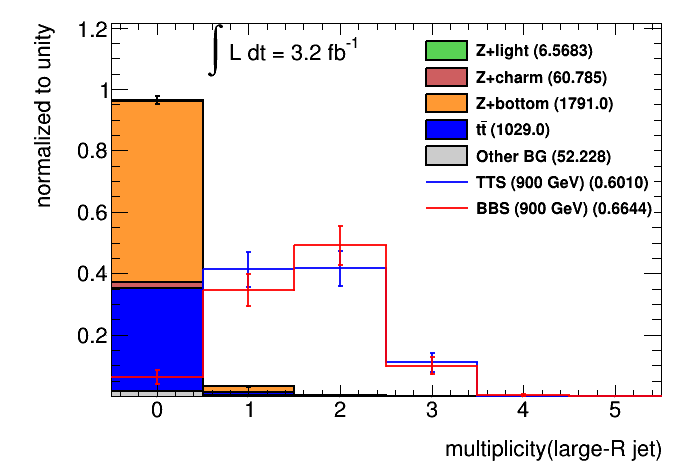
\includegraphics[width=8cm]{figures/multipliljet.png}
\caption{Plot for the large-R jet multiplicity after the preselection. 
Both signal and background are presented and the distributions are normalized to unity. 
The weighted number of events is displayed in the legend in brackets next to the processes. 
The number of events are expected for a integrated luminosity $\int L dt$ = \SI{3.2}{fb^{-1}}}
\label{ljetmult}
\end{figure}

As expected, the background processes mostly have no large-R jets because in most cases the $p_{T}$ of the particles is not high enough to produce large-R jets with the minimum requirements (see table \ref{calibration}).
The decay topology considered in this analysis gives reason to expect two large-R jets resulting from the boosted top-quark and W boson decays.
Therefore the signal distribution looks not like expected caused by the fact that about 40 \% of the events only have one large-R jets. 
An explanation for the distribution could be, that the W bosons from T \texorpdfstring{$\longrightarrow$}~Wb and B \texorpdfstring{$\longrightarrow$}~Wt  can be located in an area of $\Delta R = 1.0$ around the Z candidate and therefore are ignorated caused by the overlap removal mentioned earlier.
For the BBS signal process the case mentioned before is also possible for the jet resulting from the top quark.
Furthermore for the TTS signal process it is possible that the decay products of the W-boson and the top quark are clustered in one large-R jet because they are in an area of $\Delta R = 1.0$.\\
The requirement of two large-R jets selects the background from the signal and rejects a lot of background.
There are also a lot of signal events which are ignored as dicussed before.
A representation for the distribution of the top- and W-tag multiplicity can be found in  figure \ref{topmultipli} and \ref{bosonmultipli}.

\begin{figure}[h]
    \centering
    \resizebox{0.46\columnwidth}{!}{
    \begin{subfigure}{.49\textwidth}
      \centering
      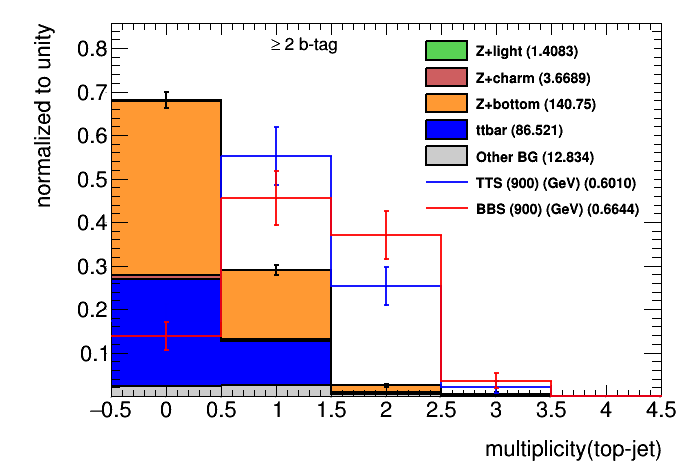
\includegraphics[width=.99\linewidth]{figures/topmultiplicity.png}
      \caption{}
      \label{topmultipli}
    \end{subfigure}
    }
    \resizebox{0.46\columnwidth}{!}{
    \begin{subfigure}{.49\textwidth}
      \centering
      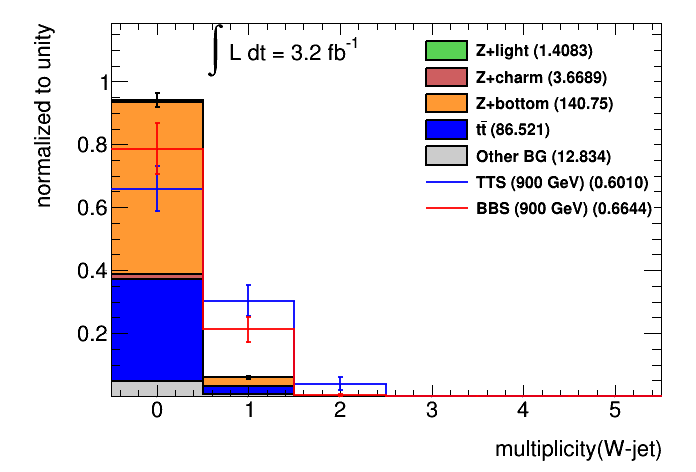
\includegraphics[width=.99\linewidth]{figures/Wmultiplicity.png}
      \caption{}
      \label{bosonmultipli}
    \end{subfigure}
    }
    \caption{Plot for the top-tagged large-R jet multiplicity (a) and W-tagged large-R jet multiplicity (b) . 
Both signal and background are presented and the distributions are normalized to unity. 
The weighted number of events is displayed in the legend in brackets next to the processes. 
The number of events are expected for a integrated luminosity $\int L dt$ = \SI{3.2}{fb^{-1}}.}
    \label{fig::stop}   
\end{figure}




The plot for the top-tag multiplicity shows that most background events do not have a top-tagged large-R jet.
That is reasonable if the Z+jets backgrounds are regarded because in these processes no top quark is included. 
The \ttbar{} process should also have no top-tag because the W bosons produced by the top quarks decay in the leptonic decay channel because there are two leptons required.
Therefore only  b-tagged jets are produced.
If the leptons resulting from the Z for the Z+jets backgrounds are not in an area $\Delta R = 1.0$ around the Z candidate they are not rejected by the overlap removal.
For the \ttbar{} process it is also possible that the leptons from the W boson decays are counted as large-R jets.
Hence there are some events with one top-tag in the background distribution.\\
The signal distribution looks not like assumed because there are a lot of events having two top-tagged large-R jets.
This is caused by the fact that the top-tagger also tag the large-R jet resulting from the W-boson as top-tag, because the lower limit for the $m_{inv}$ (mentioned in section 4.2) is at \SI{70}{GeV} for the used top-tagging working point.
The low limits for the top-tagger are chosen to avoid, that large-R jets resulting from a top, which only include the W boson, are ignored.
Figure \ref{topobosontag} shows the multiplicity fot the W-tagged jets which are not also top-tagged.

\begin{figure}[h!]
\centering
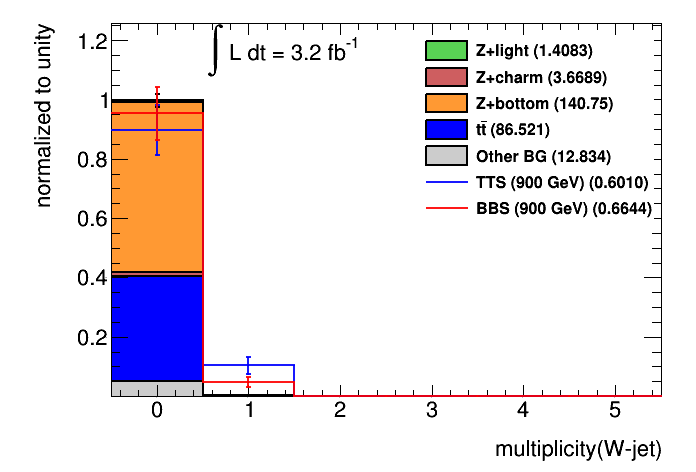
\includegraphics[width=8cm]{figures/Wotoptag.png}
\caption{Plot for the W-tag multiplicity with requiring a top-tag veto. The preselection is implemented. 
Both signal and background are presented and the distributions are normalized to unity. 
The weighted number of events is displayed in the legend in brackets next to the processes. 
The number of events are expected for a integrated luminosity $\int L dt$ = \SI{3.2}{fb^{-1}}}.
\label{topobosontag}
\end{figure}

The distribution confirms the argumentation mentioned before, because it shows that almost none W-tagged jets are not top-tagged at the same time.
The number of events without a top-tagged large-R jet can be explained with the signal efficiency of the used top-tagger.\\
The background distribution for the W-tagged large-R jets (figure \ref{bosonmultipli}) be explained with the same argumentation as for the top-tag multiplicity.
For the signal processes there is a high amount of events without W-tagged large-R jet (about 80 \% for TTS and 65 \% for BBS), which is not as expected.
This could be caused by the argumentation mentioned before that the large-R jet pruduced by the W-boson is ignored because of the overlap removal.
In addition to that the boson-tagger doesn't work perfectly but has an efficiency of 50 \%.\\
After demanding all three parts of the basic selection implied by the boosted WbZt topology, a lot of background is rejected, which becomes obvious in the three discributions described before.
The unweighted number of events, which means the real number of Monte-Carlo events, without any weights applied , and the weighted number of events (discussed in section \section{samples}) for signal and background after the basic selection is listed in table \ref{numberoevents}.
The listed numbers reveal that after the event preselection and basic selection there are for both signal and background very  low numbers of events.
An optimization study without enough statistic is not convincing because the distributions subject to large statistical uncertainties.
Therefore the optimization study in this analysis is performed without requiring at least one W-tag.
The number of events after the basic selection is much higher for both signal and background without this requirement.
These number of events both weighted and unweighted are listed in table \ref{numberoevents1}.

\begin{table}
\centering
%\setlength{\tab}{\textwidth}
\resizebox{0.8\columnwidth}{!}{
\begin{tabular}{|c|c|c|} 
\hline
\textbf{Process} & \textbf{Unweighted number of events} & \textbf{Weighted number of events}  \\
\hline
\hline
Z+light & 3 & 0.0005\\
Z+charm & 2 & 0.0060\\
Z+bottom & 77 & 0.1680\\
ttbar{} & 6 & 0.3739\\
Other BG & 1331 & 0.3298\\
TTS & 214 & 0.1094\\
BBS & 176 & 0.1089\\
\hline
\end{tabular}
}
\caption{Unweighted and weighted number of events for signal and background processes after requiring two large-R jets and both top- and W-tag.}
\label{numberoevents}
\end{table}




\begin{table}
\centering
%\setlength{\tab}{\textwidth}
\resizebox{0.8\columnwidth}{!}{
\begin{tabular}{|c|c|c|} 
\hline
\textbf{Process} & \textbf{Unweighted number of events} & \textbf{Weighted number of events}  \\
\hline
\hline
Z+light & 37 & 1.1638\\
Z+charm & 4 & 0.0668\\
Z+bottom & 849 & 6.0273\\
ttbar{} & 41 & 2.3774\\
Other BG & 6260 & 1.6494\\
TTS & 560 & 0.2922\\
BBS & 530 & 0.3856\\
\hline
\end{tabular}
}
\caption{Unweighted and weighted number of events for signal and background processes after requiring two large-R jets and at least one top-tag.}
\label{numberoevents1}
\end{table}

 



















% kapitel5.tex
\chapter{Optimization Studies for the Event Selection}

\section{Search for Discriminating Variables }
The first part of the optimization studies is the search for variables which provide a significant distinction between background and signal.
Caused by the basic selection discussed in section \ref{basic selection} there is already much background rejected.
Moreover the requirement of two large-R jets cause that the remaining background events contain high energies, because large-R jets, which fulfill the minimum criteria, have to be produced.
This complicates the search for discriminating variables, because the signal is expected to contain high energies,too, because of the massive vector-like quarks.\\
Figure \ref{H_T} shows the distribution for the scalar sum of the transverse momenta of all jets in an event.

\begin{figure}
\centering
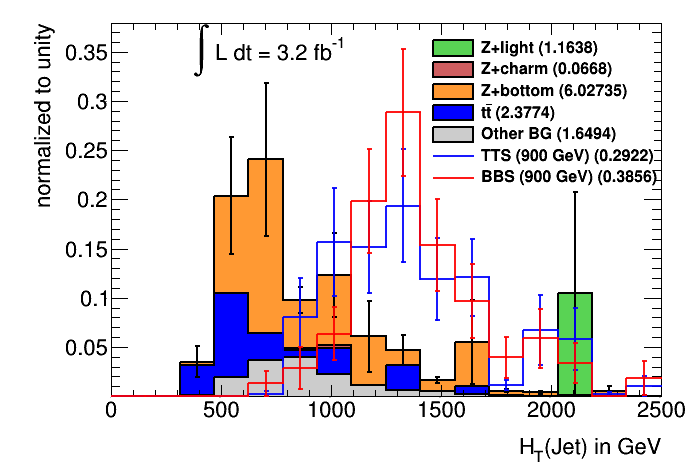
\includegraphics[width=8cm]{figures/H_T.png}
\caption{Plot for the scalar sum of all jet $p_{T}$'s in an event after the preselection. 
Both signal and background are presented and the distributions are normalized to unity. 
The weighted number of events is displayed in the legend in brackets next to the processes. 
The number of events are expected for a integrated luminosity $\int L dt$ = \SI{3.2}{fb^{-1}}}
\label{H_T}
\end{figure}

The distribution shows, that the signal is shifted to the right compared to the background, because there is more energy in the events resulting from the very massive vector-like quarks. 
Figure \ref{Zpt} presents the distribution of the Z candidate $p_{T}$.
\begin{figure}
\centering
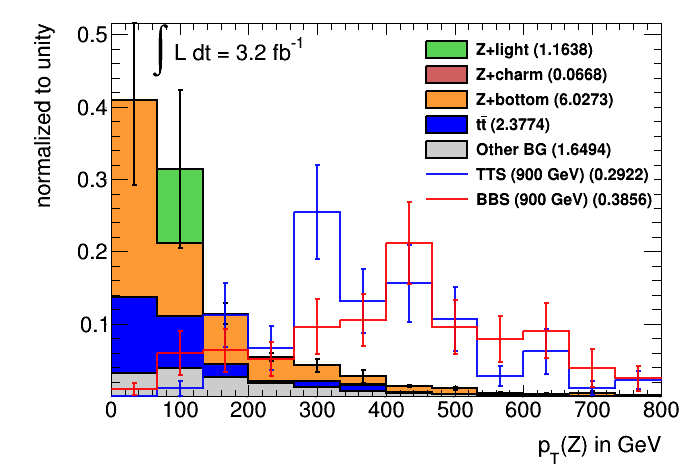
\includegraphics[width=8cm]{figures/Zpt.png}
\caption{Plot for the Z candidate $p_{T}$. 
Both signal and background are presented and the distributions are normalized to unity. 
The weighted number of events is displayed in the legend in brackets next to the processes. 
The number of events are expected for a integrated luminosity $\int L dt$ = \SI{3.2}{fb^{-1}}}
\label{Zpt}
\end{figure}

As mentioned for the $H_{T}$-distribution the signal is shifted to the right. That is as expeced, because the Z candidate results straight from the vector-like quark and should have a $p_{T}$ about \SI{450}{GeV}.
In figure \ref{leadingljet} the $p_{T}$ of the leading large-R jet is represented, which means the $p_{T}$ of the large-R jets with the highest $p_{T}$ in an event.
\vspace{-0.5cm}
\begin{figure}[h!]
\centering
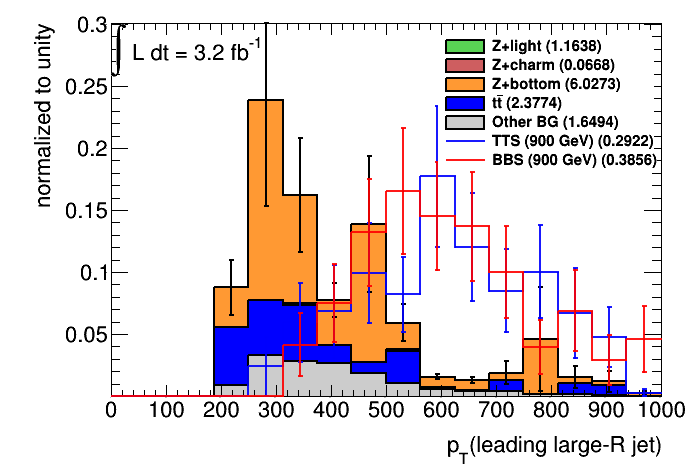
\includegraphics[width=8cm]{figures/leadingljet.png}
\caption{Plot for the leading large-R jet $p_{T}$. 
Both signal and background are presented and the distributions are normalized to unity. 
The weighted number of events is displayed in the legend in brackets next to the processes. 
The number of events are expected for a integrated luminosity $\int L dt$ = \SI{3.2}{fb^{-1}}.}
\label{leadingljet}
\end{figure}

Figure \ref{mZb} shows the distribution of the invariant mass of the Z candidate and the highest $p_{T}$ b-jet and \ref{mZt} the invariant mass of the Z candidate and the highest $p_{T}$ top-jet.


%\resizebox{0.48\columnwidth}{!}{
\begin{figure}[h]
    \centering
    \resizebox{0.46\columnwidth}{!}{
    \begin{subfigure}{.49\textwidth}
      \centering
      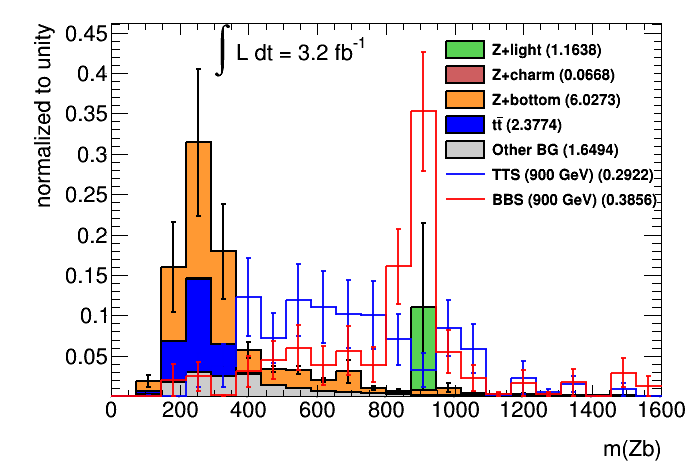
\includegraphics[width=.99\linewidth]{figures/mZb.png}
      \caption{}
      \label{mZb}
    \end{subfigure}
    }
    \resizebox{0.46\columnwidth}{!}{
    \begin{subfigure}{.49\textwidth}
      \centering
      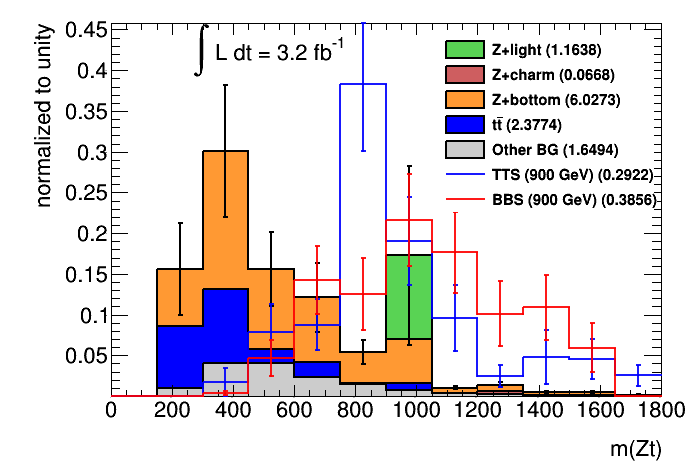
\includegraphics[width=.99\linewidth]{figures/mZt.png}
      \caption{}
      \label{mZt}
    \end{subfigure}
    }
    \caption{Plot for the invariant mass of the Z candidate and the highest $p_{T}$ b-jet (a) and the invariant mass of the Z candidate and the highest $p_{T}$ top-jet (b)  . 
Both signal and background are presented and the distributions are normalized to unity. 
The weighted number of events is displayed in the legend in brackets next to the processes. 
The number of events are expected for a integrated luminosity $\int L dt$ = \SI{3.2}{fb^{-1}}.}
    \label{fig::stop}   
\end{figure}
%}
The signal is shifted to the right caused by the same argumentation mentioned before. 
For the BBS signal process there is a peak at \SI{900}{GeV} in figure \ref{mZb}.
This is as expected because the Z candidate and the highest $p_{T}$ b-jet should result from the vector-like quark decay B \texorpdfstring{$\longrightarrow$}~Zb.
For the peak 


\section{Significance for Different Cuts}

\section{Proposel for a Boosted Event Selection}


% kapitel6.tex
\chapter{Summary and Conclusions}



\appendix
% Hier beginnt der Anhang, nummeriert in lateinischen Buchstaben
\chapter{Ein Anhangskapitel}

Hier könnte ein Anhang stehen, falls Sie z.B. Code, Konstruktionszeichnungen oder ähnliches mit in die Arbeit bringen wollen. Im Normalfall stehen jedoch alle Ihre Resultate im Hauptteil der Bachelorarbeit und ein Anhang ist überflüssig.


\backmatter
\printbibliography

\cleardoublepage
\thispagestyle{empty}
\section*{Eidesstattliche Versicherung}
Ich versichere hiermit an Eides statt, dass ich die vorliegende Abschlussarbeit mit dem Titel \enquote{\thetitle} selbstständig und ohne unzulässige fremde Hilfe erbracht habe.
Ich habe keine anderen als die angegebenen Quellen und Hilfsmittel benutzt, sowie wörtliche und sinngemäße Zitate kenntlich gemacht. 
Die Arbeit hat in gleicher oder ähnlicher Form noch keiner Prüfungsbehörde vorgelegen.

\vspace*{1cm}\noindent
\begin{center}
  \begin{tabular}{@{}p{0.4\textwidth}@{\hspace{0.15\textwidth}}p{0.4\textwidth}@{}}
  \rule{\linewidth}{0.25pt}& \rule{\linewidth}{0.25pt}\\
  Ort, Datum & Unterschrift
  \end{tabular}
\end{center}

\subsection*{Belehrung}
Wer vorsätzlich gegen eine die Täuschung über Prüfungsleistungen betreffende Regelung einer Hochschulprüfungsordnung verstößt, handelt ordnungswidrig.
Die Ordnungswidrigkeit kann mit einer Geldbuße von bis zu \SI[round-mode=places, round-precision=2]{50000}{€} geahndet werden. 
Zuständige Verwaltungsbehörde für die Verfolgung und Ahndung von Ordnungswidrigkeiten ist der Kanzler/die Kanzlerin der Technischen Universität Dortmund. 
Im Falle eines mehrfachen oder sonstigen schwerwiegenden Täuschungsversuches kann der Prüfling zudem exmatrikuliert werden \mbox{(\S\,63 Abs. 5 Hochschulgesetz --HG--).}

Die Abgabe einer falschen Versicherung an Eides statt wird mit Freiheitsstrafe bis zu 3 Jahren oder mit Geldstrafe bestraft.

Die Technische Universität Dortmund wird ggf.\ elektronische Vergleichswerkzeuge (wie z.\,B.\ die Software \enquote{turnitin}) zur Überprüfung von Ordnungswidrigkeiten in Prüfungsverfahren nutzen. \\[\baselineskip]

\noindent Die oben stehende Belehrung habe ich zur Kenntnis genommen.\\[1cm]
\begin{center}
\begin{tabular}{@{}p{0.4\textwidth}@{\hspace{0.15\textwidth}}p{0.4\textwidth}@{}}
\rule{\linewidth}{0.25pt}& \rule{\linewidth}{0.25pt}\\
Ort, Datum & Unterschrift
\end{tabular}
\end{center}

\end{document}
